\begin{frame}{Coupling mechanisms}

    \begin{columns}[T] 
        \begin{column}{0.32\textwidth}
            \centering
            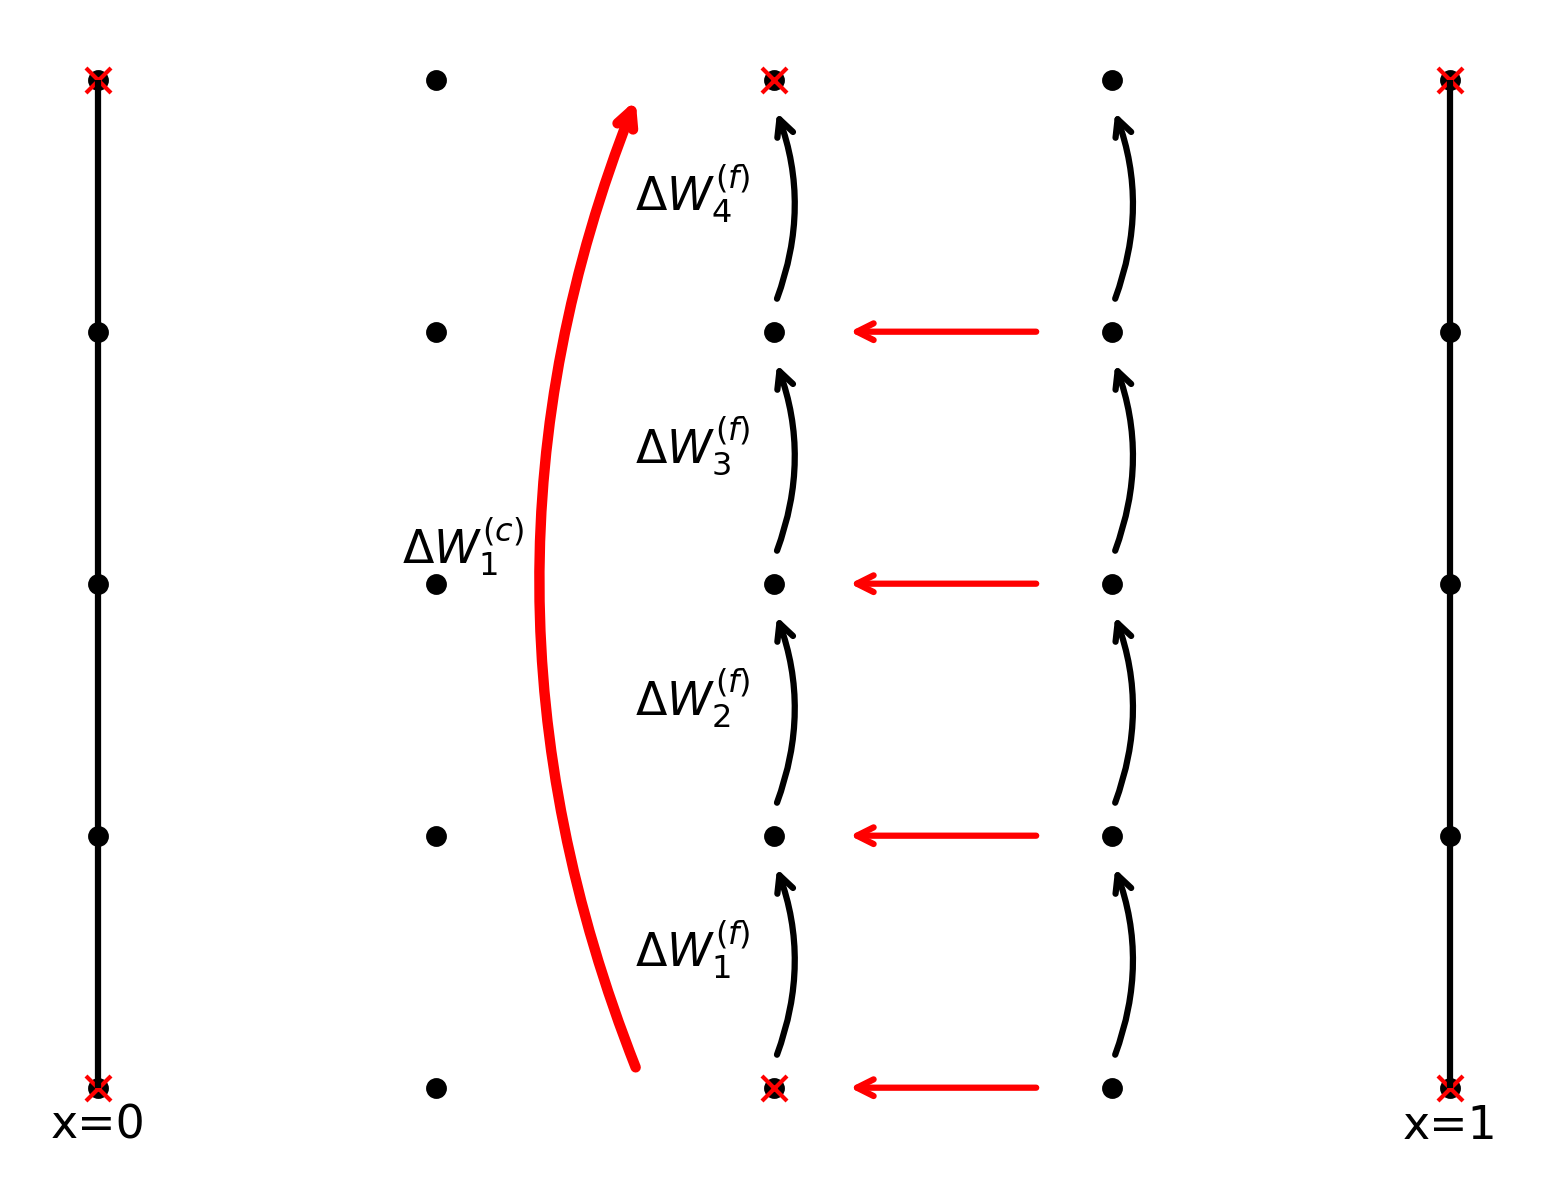
\includegraphics[width=\linewidth]{presentation_graphics/nn.png}
            {Nearest-Neighbour}
            \begin{itemize}\tiny
                \item Used by Cornalba \& Fischer.
                \item Coarse noise = sum of underlying + fine neighbour.
            \end{itemize}
        \end{column}

        \begin{column}{0.32\textwidth}
            \centering
            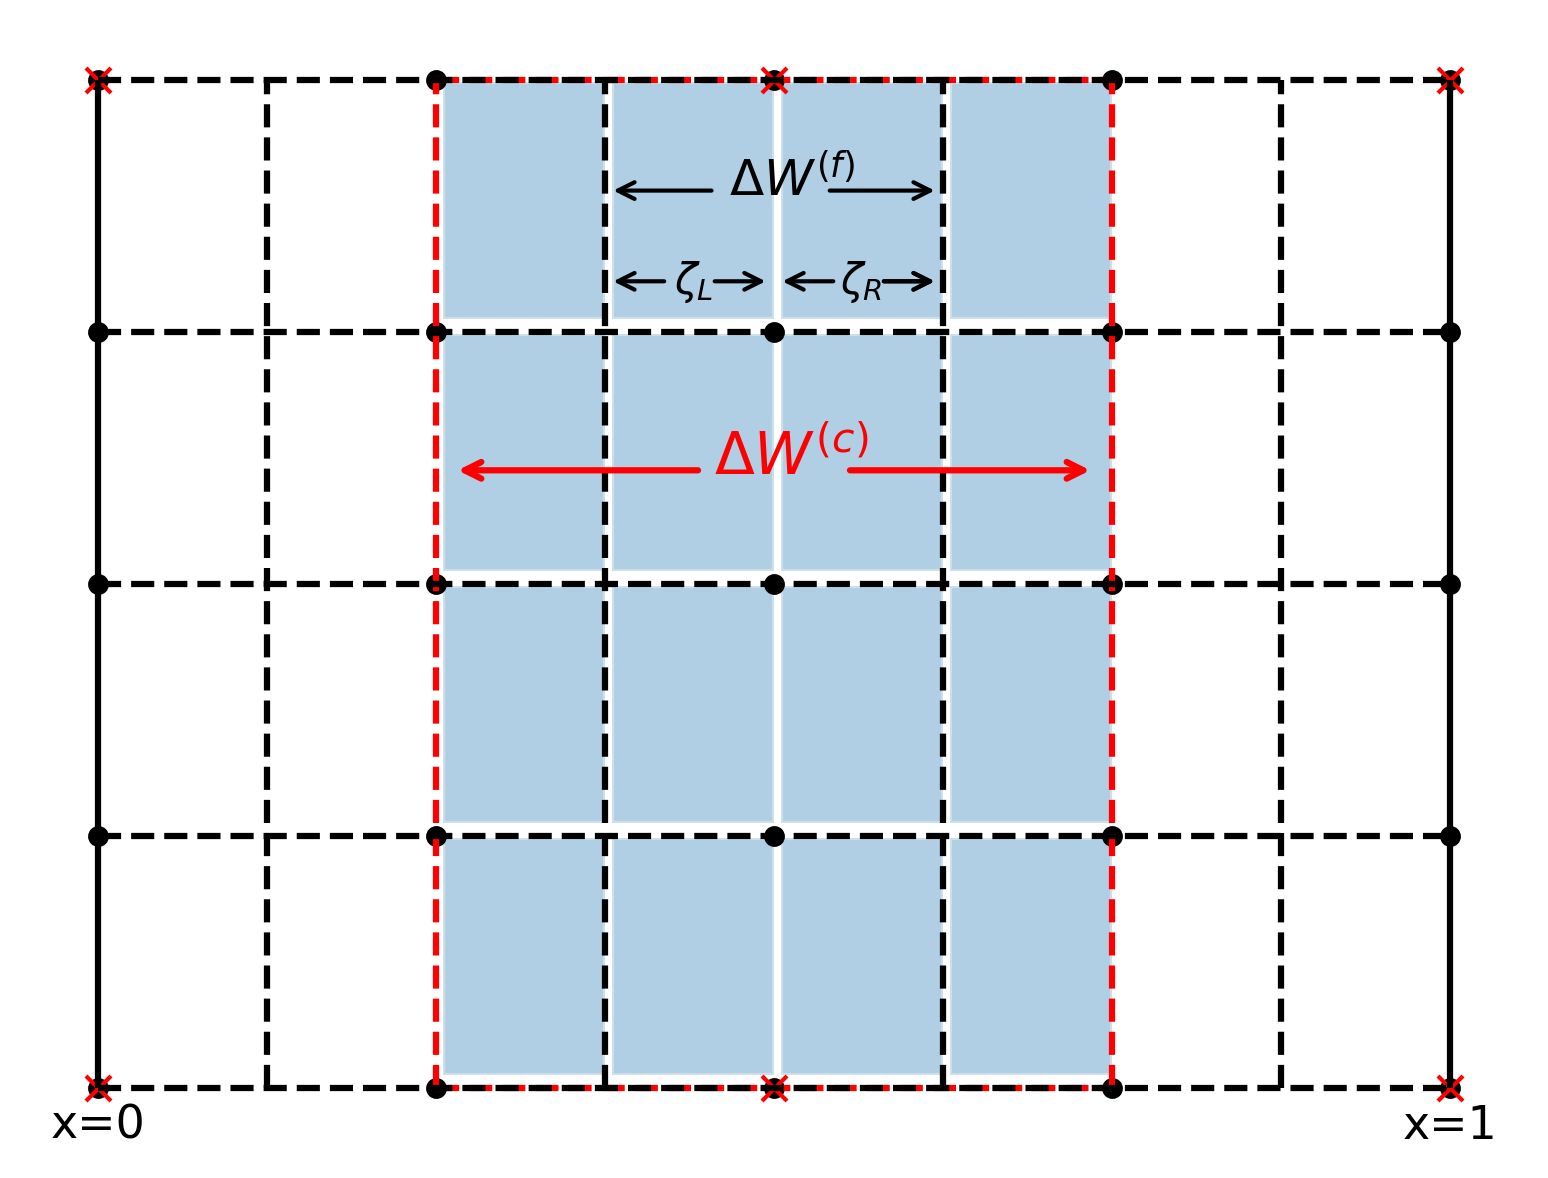
\includegraphics[width=\linewidth]{presentation_graphics/cc.png}
            {Central Coupling}
            \begin{itemize}\tiny
                \item Introduced in this dissertation.
                \item Mesh split into half-cells.
                \item Coarse noise built from shared half-cell increments.
            \end{itemize}
        \end{column}

        \begin{column}{0.32\textwidth}
            \centering
            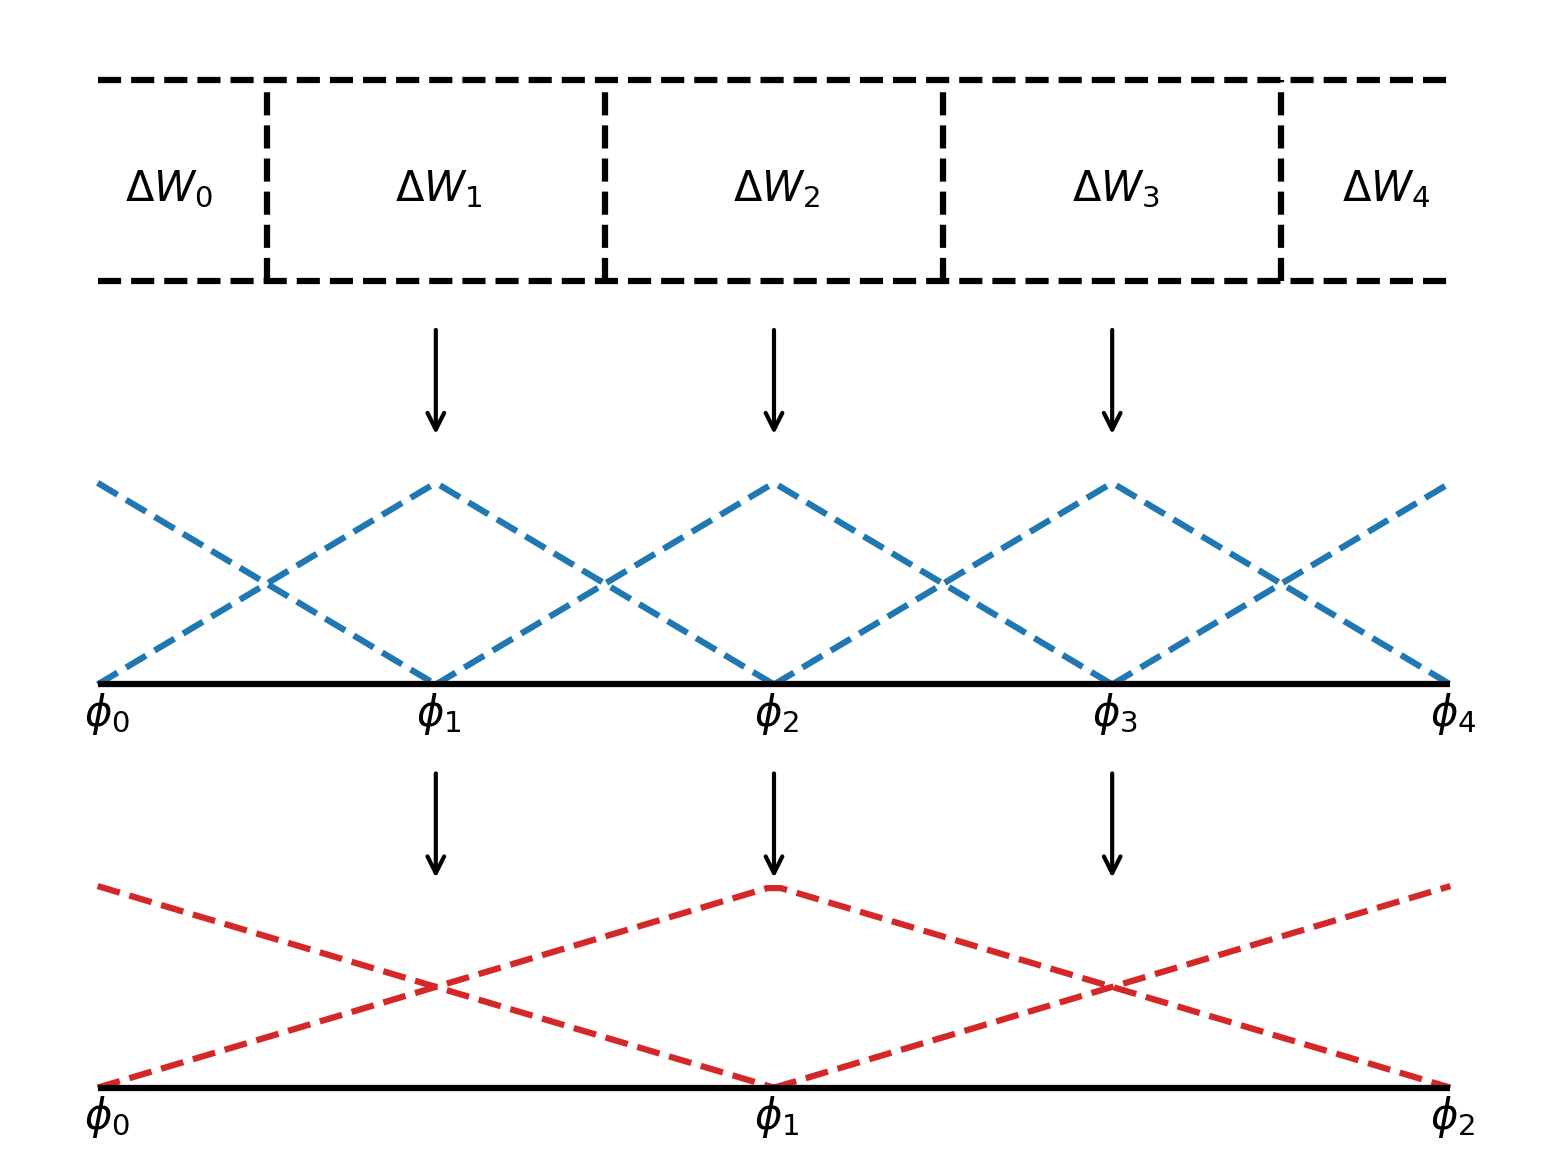
\includegraphics[width=\linewidth]{presentation_graphics/fe.png}
            {Finite Element}
            \begin{itemize}\tiny
                \item Introduced in this dissertation.
                \item Noise projected onto hat basis.
                \item Coarse hats formed as sums of fine hats.
            \end{itemize}
        \end{column}
    \end{columns}

    \begin{textblock*}{9cm}(4.9cm,5.25cm)
        \scalebox{0.4}{
            $t_c = 0,
            t_f = 0$
        }
    \end{textblock*}
    \begin{textblock*}{9cm}(4.9cm,2.35cm)
        \scalebox{0.4}{
            $t_c = 1, t_f = 4$
        }
    \end{textblock*}
\end{frame}

